\chapter{Evaluations} \label{ch:result}
\begin{figure}[H]
\centering
\caption{Simulation of the dataset}
\includegraphics[width=0.5\linewidth,scale=0.25]{figures/dataset}
\label{fig:dataset}
\end{figure}
The INTERACTION Dataset \footnote{https://interaction-dataset.com/} is used to evaluate the algorithms. The dataset contains multiple scenarios in different locations, captured using drones or fixed cameras over a variable amount of time. Each scenario consists of multiple traffic participants, identified by an ID, and each frame per 0.1s has a set of vehicles and their position and velocity in the x and y-direction. Over a choice of multiple videos, the location with all videos summing up to a total length of 259.43 minutes is chosen for this paper. A simulated scenario is demonstrated in Fig.~\ref{fig:dataset}. There are 60 recorded files in this location with a total of 10,518 vehicles. The position in the x and y-direction is used as a measurement input to the algorithms, whereas the velocity in the x and y-direction is used to calculate the error and evaluate the estimates. 

With every participant modeled as \eqref{formula:system}, the initial state is set as \eqref{eq:initial}. The matrices $E$ and $F$ are $I_{n_x}$ and $I_{n_y}$ respectively. All zonotopes are limited to maximum order of $20$. 
\begin{equation}
\label{eq:initial}
\begin{split}
\mathcal{X}_0 &= \langle 0, diag([1000\quad 1000\quad 10 \quad10\quad 10\quad 10]^T) \rangle\\
\overline{w_k} &= [0.1\quad 0.1\quad 0.4\quad 0.4\quad 0.1\quad 0.1]^T\\
\overline{v_k} &= [0.1\quad 0.1]^T
\end{split}
\end{equation}

All the evaluation are carried out by single-threaded scripts run on an Intel(R) Core(TM) i7-7500U CPU @ 2.70GHz machine with MATLAB\textsuperscript{\tiny\textregistered} 2019b. The CORA toolbox is used for set computations; the Mosek solver in YALMIP toolbox is used to solve the optimization problems. Templates to implement model and estimator in MATLAB\textsuperscript{\tiny\textregistered} is attached in the Appendix~\ref{app:code}.

\section{Computation Time}
\begin{figure}[H]
\centering
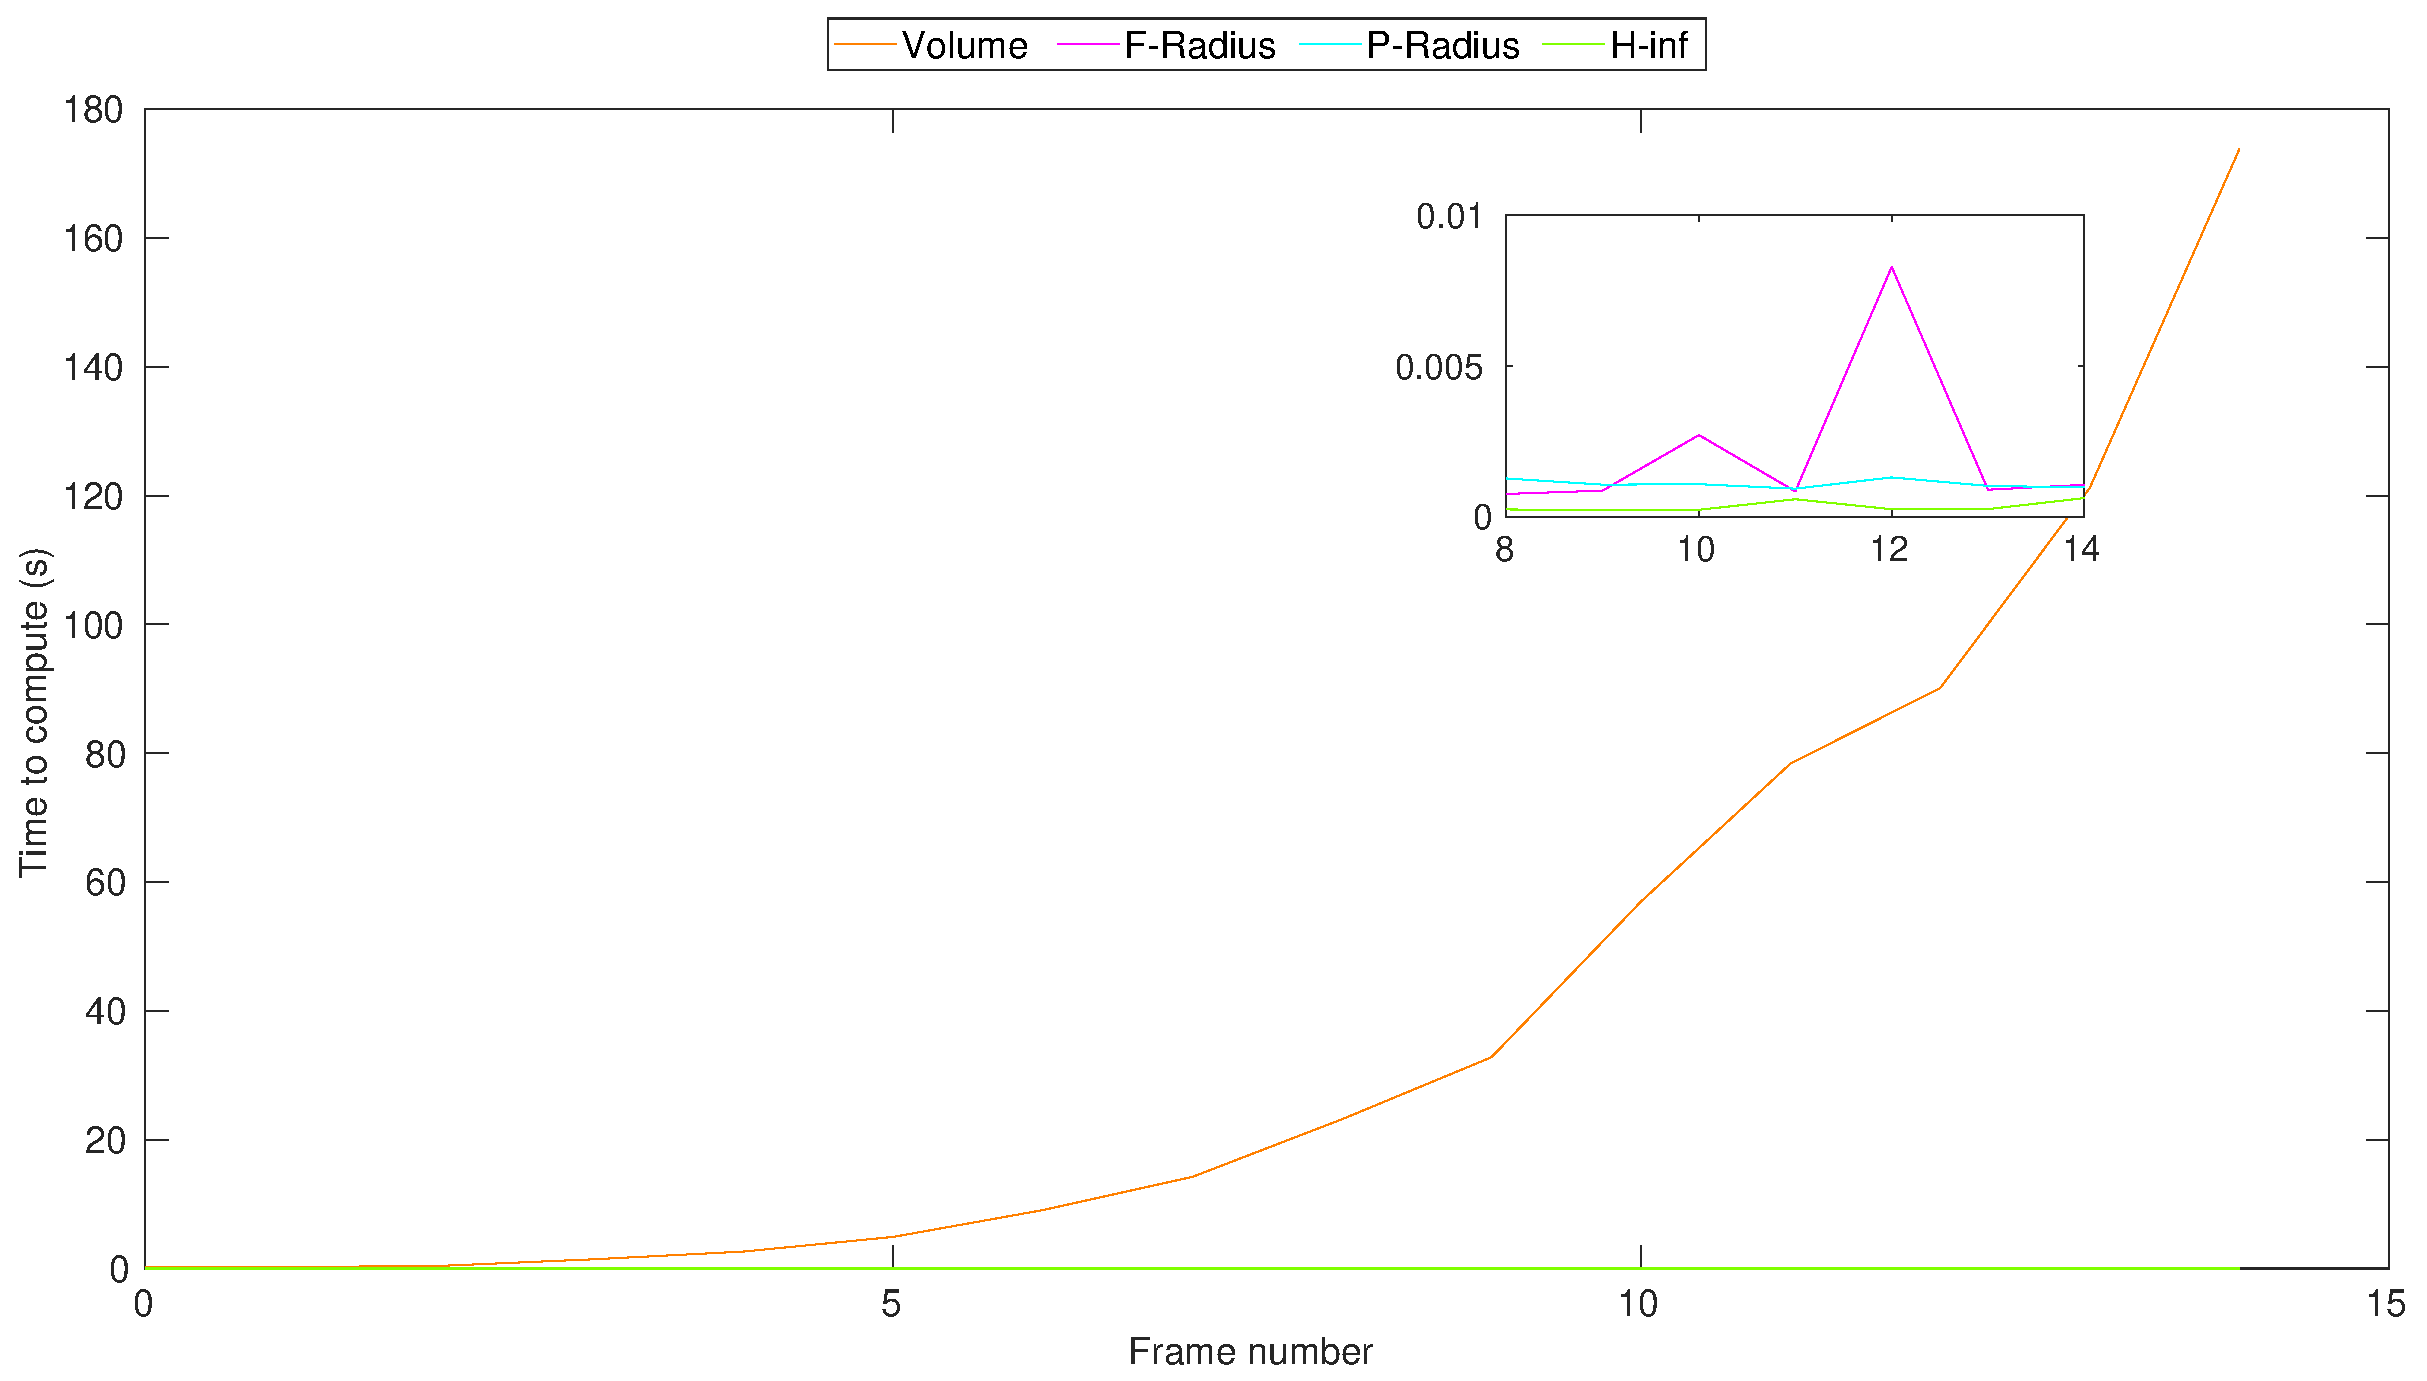
\includegraphics[width=\linewidth]{figures/timegraphh}
\caption{Computation time for each method to estimate using the CV model}
\label{fig:timegraph}
\end{figure}
Fig.~\ref{fig:timegraph} illustrates that the computation time for volume minimization rises exponentially over time. Due to the choice of limiting zonotope order to $m\leq20$, the time for volume computation is expected to steeply rise till the $16^{th}$ frame for the cv model. As seen from the figure, the computation time has reached 16,000\% of the time step. Such an outcome makes volume minimization futile for a collision avoidance system; hence this method is avoided in the rest of the paper.

\begin{table}[!h]
\caption{Comparison of computation time (ms)\\}
	\centering
	\renewcommand{\arraystretch}{1.1}
	\small	
	\begin{tabular}{l l l l}
		\toprule
		& \multicolumn{3}{c}{\textbf{Average Computation Time (ms)}}\\
		\textbf{Method} & CV model & CA model & PM model\\ \midrule
		%-------------------------------------		
		F-Radius & 0.396 & 0.375 & 0.621 \\
		P-Radius & 0.312 & 0.319 & 0.544\\
		H-$\infty$ approximation & 0.145 & 0.147 & 0.144\\
		%--------------------------------------		
		\bottomrule
	\end{tabular}
	\label{tab:comptime}
\end{table}
Tab. \ref{tab:comptime} shows that the computation time for the other methods is negligible compared to the frame rate, i.e 100ms. Furthermore, the H-$\infty$-based interval observer has almost half the time taken by the segment intersection methods, which can be explained by the absence of zonotope reduction operation in the former method. 

In addition, Tab.~\ref{tab:comptime} highlights how the choice of vehicle model affects the performance. The H-$\infty$-based observer is not much affected by models, whereas, the segment minimization methods have a significant decline in performance with the point-mass model. This observation can be explained by how the constraints in the point-mass model are applied. In segment minimization methods, the point-mass model applies constraints on the zonotope for the state, whereas, the H-$\infty$-based observer only constraints the upper and lower bound. 

\section{Time to Converge}
\begin{table}[!h]
\caption{Comparison of approximate time (in s) to converge}
	\centering
	\renewcommand{\arraystretch}{1.1}
	\small	
	\begin{tabular}{l l l l l l}
		\toprule 
		
		& \multicolumn{3}{c}{\textbf{Velocity}} & \multicolumn{2}{c}{\textbf{Acceleration}}\\ \cmidrule(l){2-4} \cmidrule(l){5-6}
		\textbf{Method} & \textbf{CV model} & \textbf{CA model} & \textbf{PM model} & \textbf{CA model} & \textbf{PM model}\\ \midrule
		%-------------------------------------		
		F-Radius & 0.2 & 0.2 & 0.2 & 0.6 & 4.3\\
		P-Radius & 4.8 & 3.7 & 3.7 & 5 & 5.2 \\
		H-$\infty$ approximation & 1.5 & 2.9 & 2.8 & 3.2 & 3.6\\
		%--------------------------------------		
		\bottomrule
	\end{tabular}
	\label{tab:convtime}
\end{table}
The time to converge is an important performance metric but is difficult to measure. For this paper, it is calculated as the time taken for the rate of change of estimated bounds to approach zero. Tab.~\ref{tab:convtime} shows the approximate time for $velocity_x$ and $acceleration_x$ estimates to converge. It is trivial to note that the P-radius technique demonstrates the worst performance, which can be explained by its fixed pre-computed parameter for the intersected segment. In contrast, the F-radius technique, which adjusts the aforementioned parameter in run-time for every measurement, performs the best, taking at most six time steps (compared to fifty time steps for P-radius minimizer) to converge both velocity and acceleration. An exception appears in the pm model, which can be explained by the disturbance in model linearity due to its constraint in acceleration. 

In general, the point-mass model delays the time to converge. Interestingly, the H-$\infty$-based observer exhibit a rather consistent time to converge, even for an increase in state dimension (e.g. ca model) or new constraints (e.g. pm model). This behavior makes H-$\infty$-based observer apt for complex models. An extended result of the rate of change of bounds of all the variables over time is available in the Appendix~\ref{eresult:rate}. 

\section{Bounds}
\begin{figure}[h]
\centering \includegraphics[scale=0.8]{figures/legend}\\
\begin{subfigure}{0.32\textwidth}
\centering
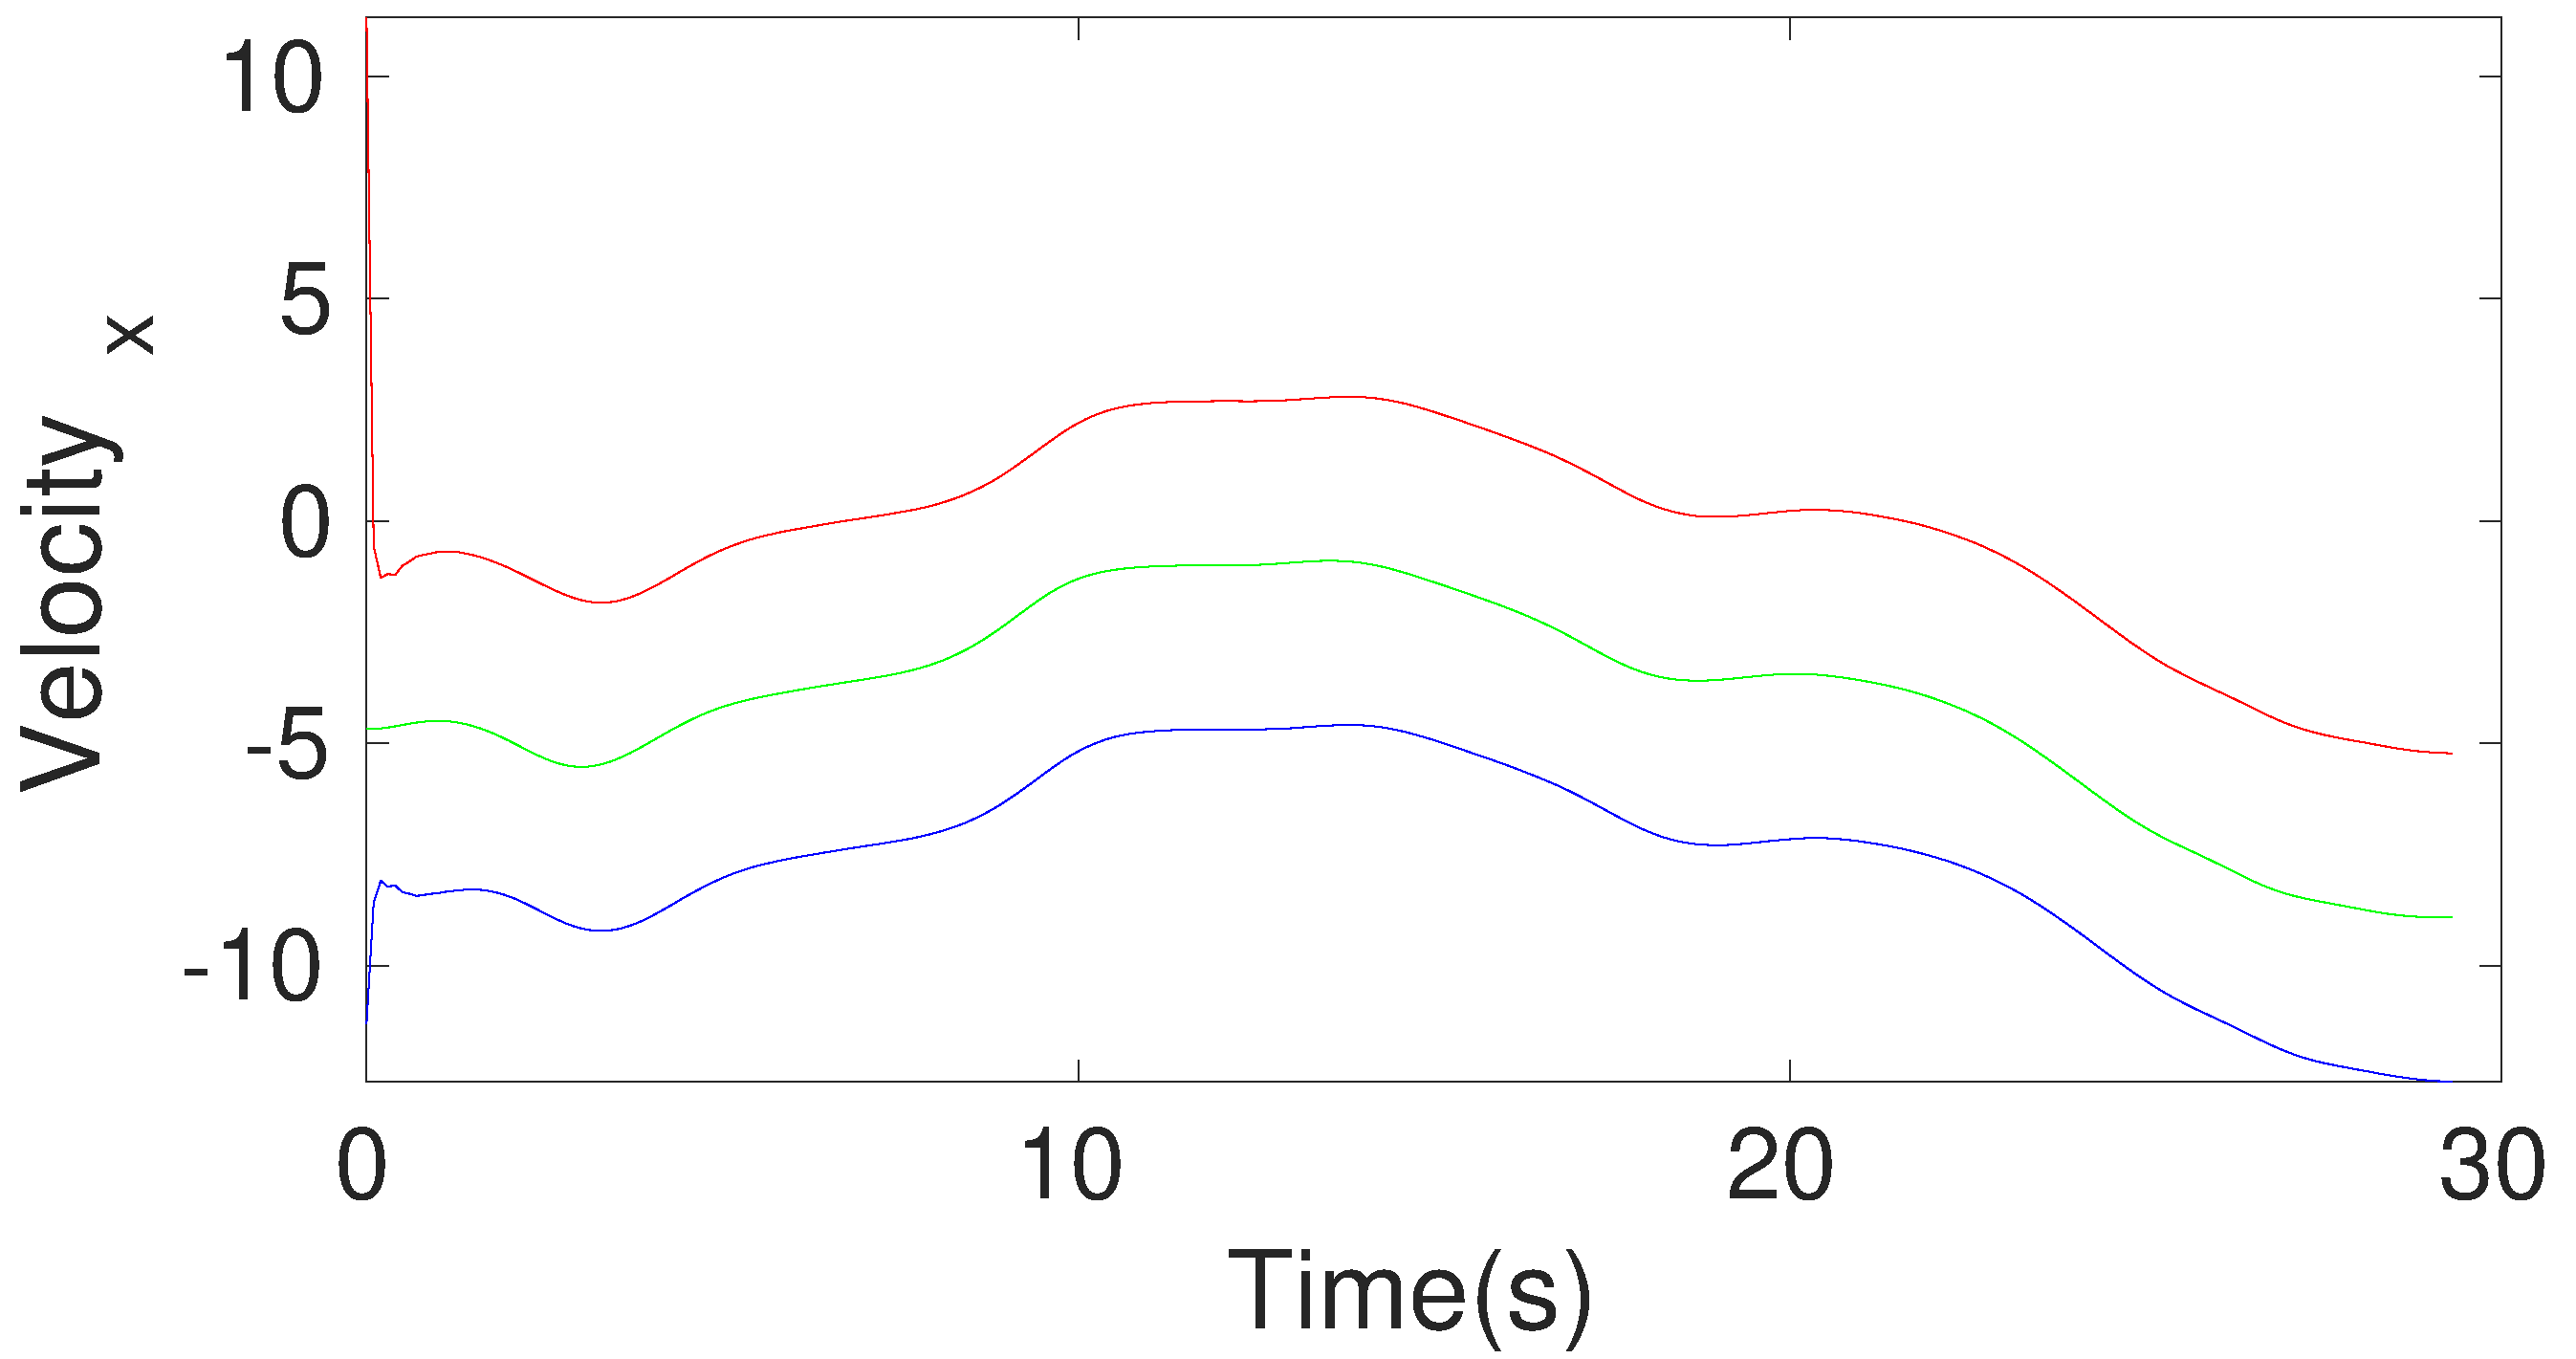
\includegraphics[width=\linewidth]{figures/sm}\caption{F-radius minimizer}
\end{subfigure}
\begin{subfigure}{0.32\linewidth}
\centering
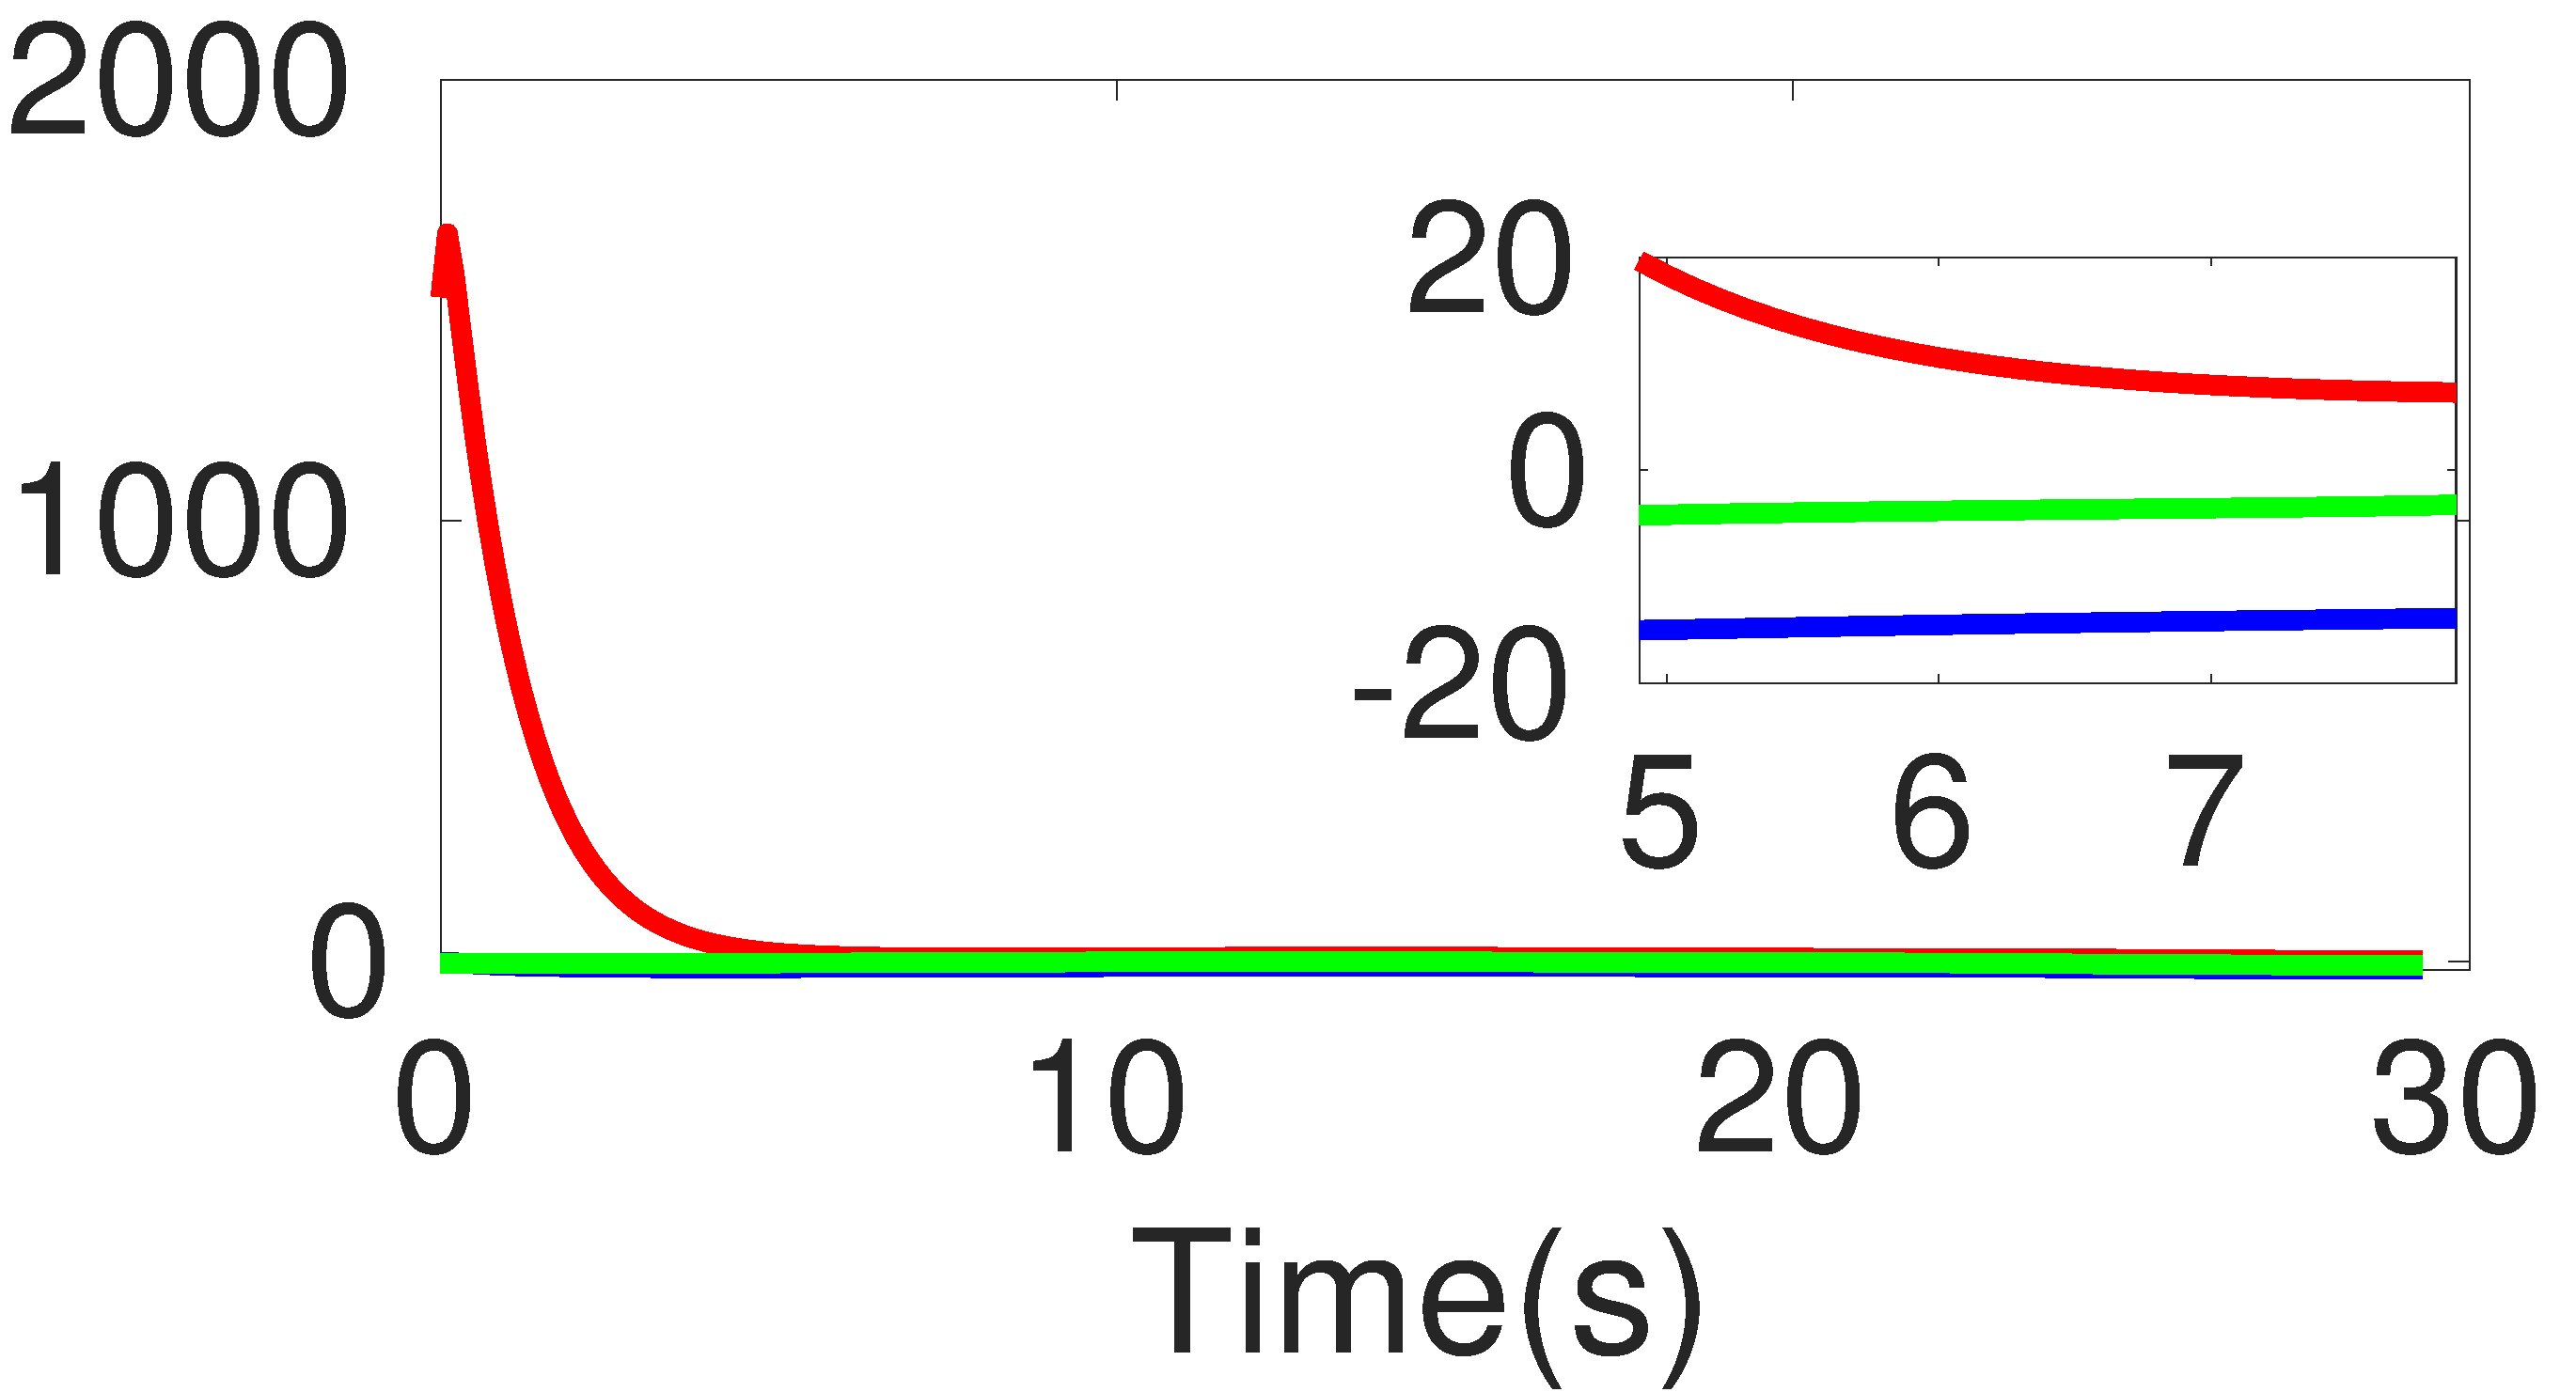
\includegraphics[width=\linewidth]{figures/prad}\caption{P-radius minimizer}
\end{subfigure}
\begin{subfigure}{0.32\linewidth}
\centering
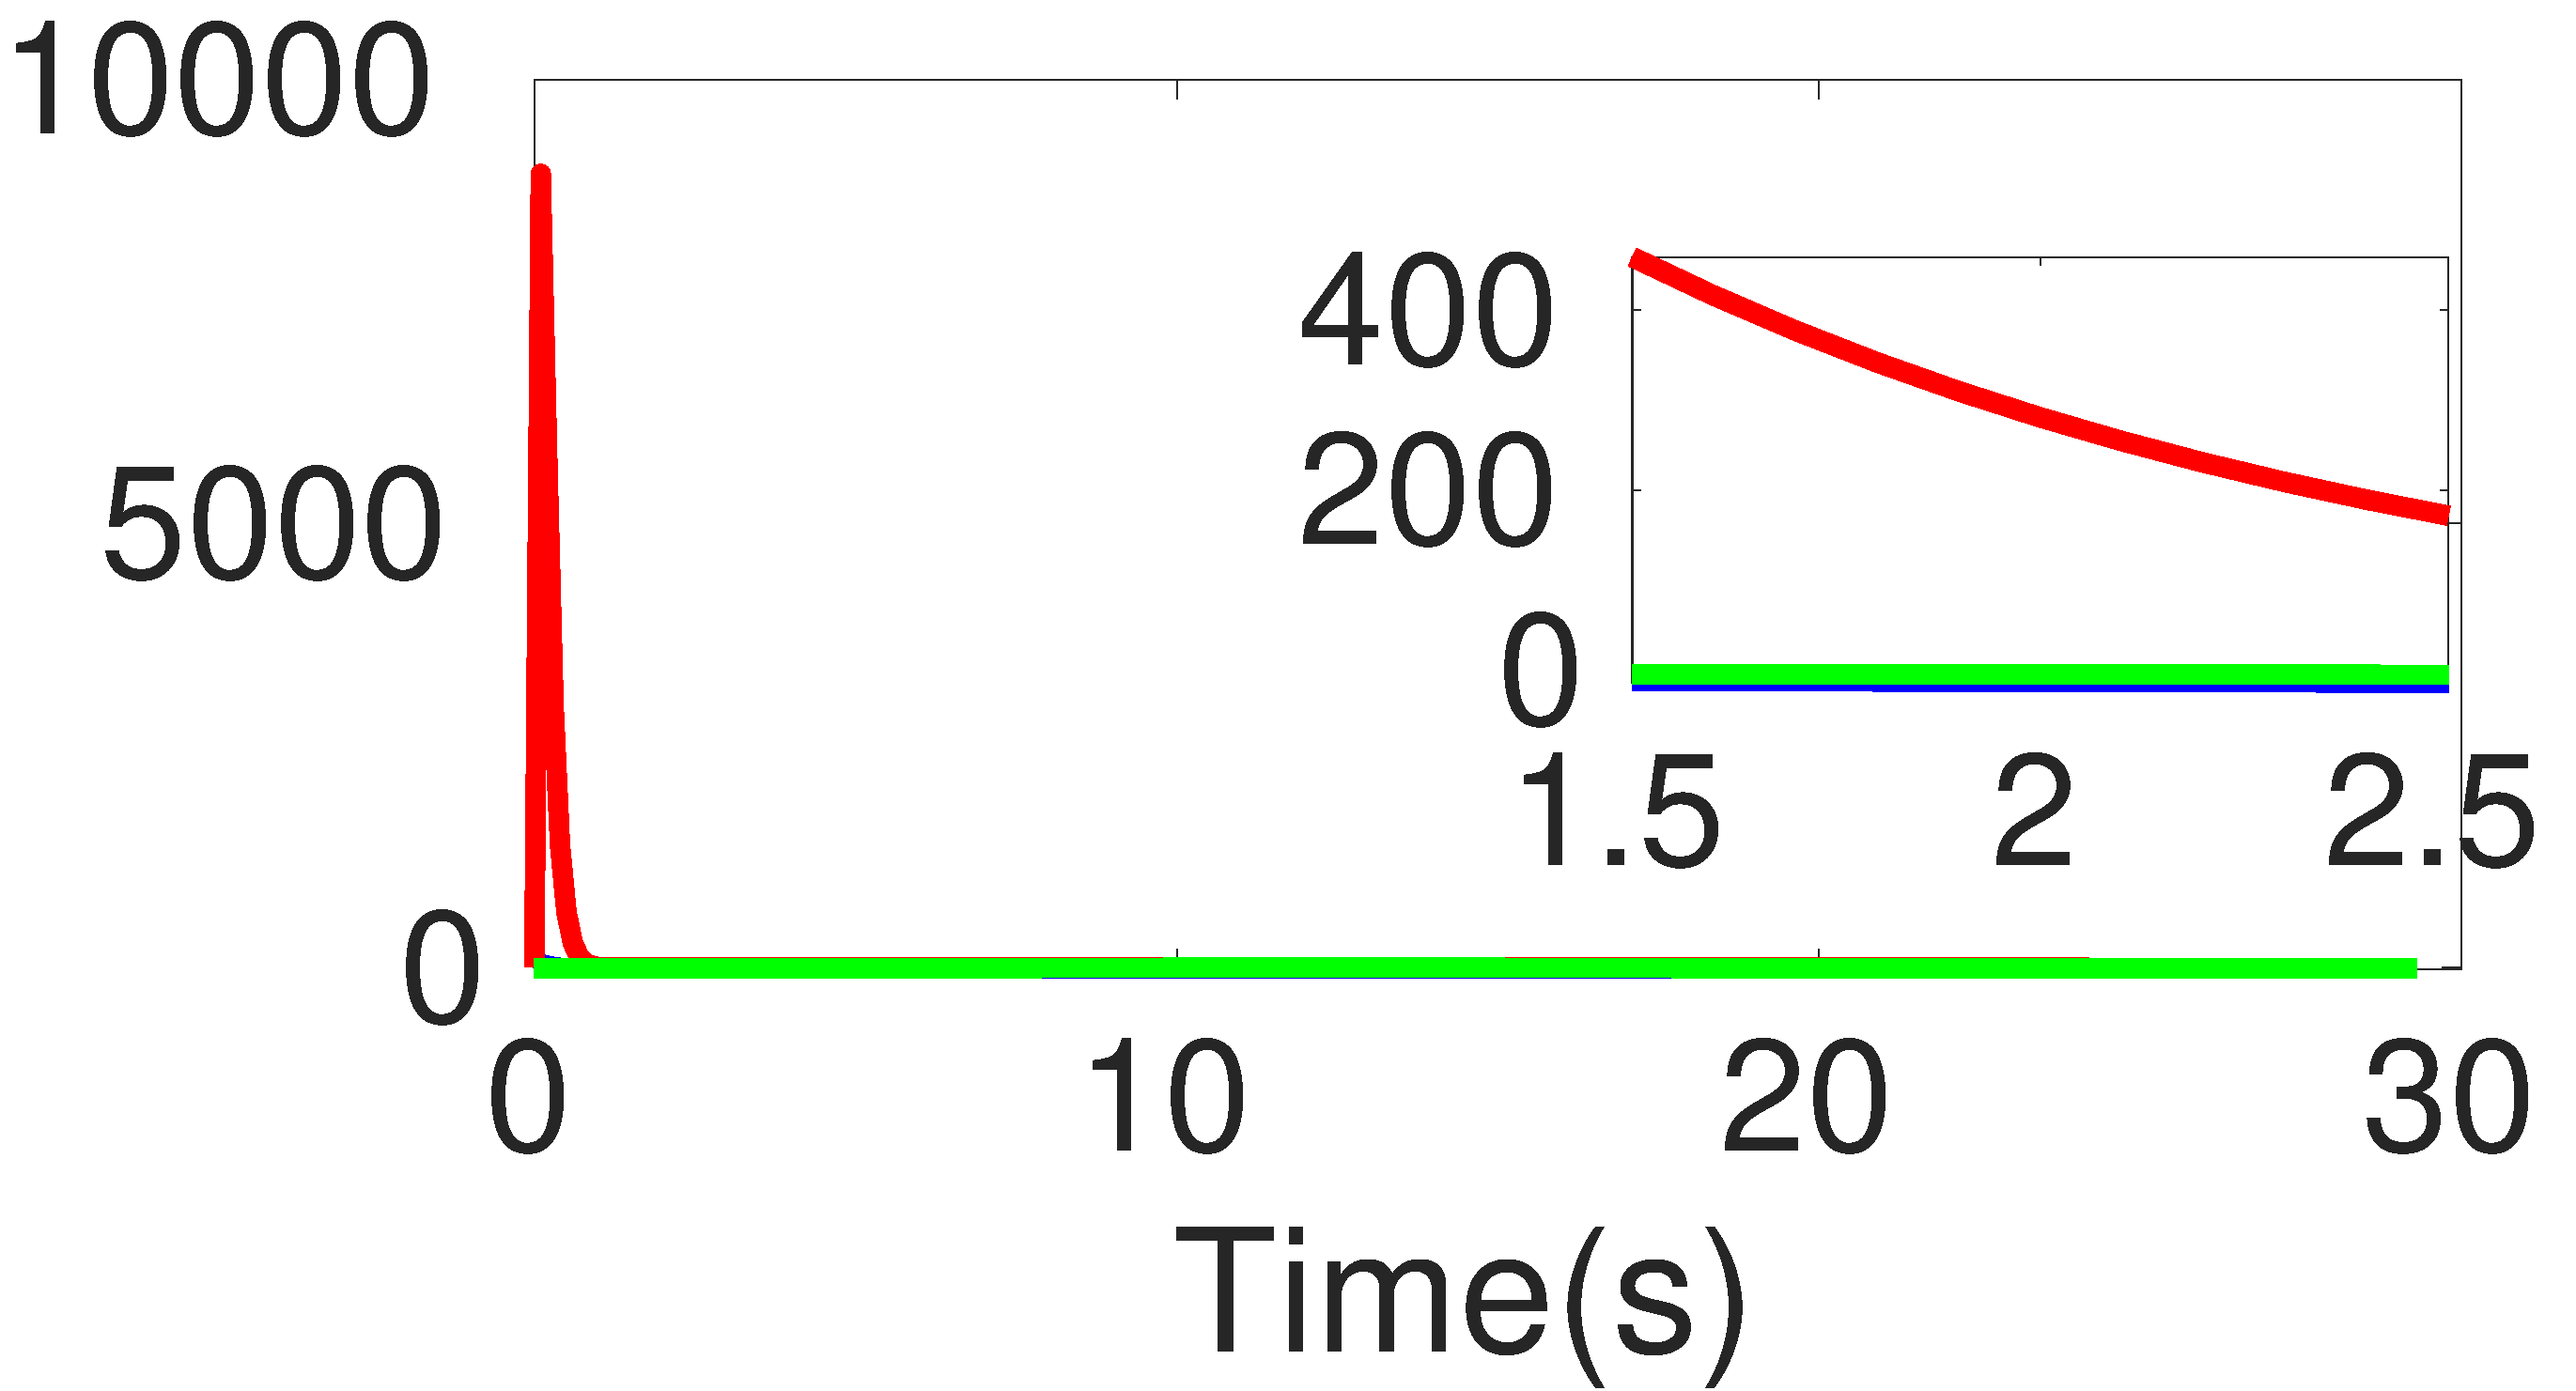
\includegraphics[width=\linewidth]{figures/hinf}\caption{H-$\infty$-based observer}
\end{subfigure}
\caption{The $velocity_x$ bounds using pm model}
\label{fig:bound}
\end{figure}
\begin{table}[htbp]
\caption{Comparison of bounds of estimation\\}
	\centering
	\renewcommand{\arraystretch}{1.1}
	\small	
	\begin{tabular}{l l l l l l l}
		\toprule 
		& \multicolumn{6}{c}{\textbf{Constant Velocity}}\\
		\textbf{Method} & \textbf{$s_x$} & \textbf{$s_y$} & \textbf{$v_x$} & \textbf{$v_y$} & \textbf{$a_x$} & \textbf{$a_y$}\\ \midrule
		%-------------------------------------		
		F-Radius & 0.441 & 0.441 & 5.686 & 5.686 & - & -\\
		P-Radius & 0.4606 & 0.459 & 13.45 & 13.45 & - &	-\\
		H-$\infty$ approximation & 0.9867 &	0.937 &	6.177 & 6.177 & - &-\\
		
		& \multicolumn{6}{c}{\textbf{Constant Acceleration Model}}\\
		 & \textbf{$s_x$} & \textbf{$s_y$} & \textbf{$v_x$} & \textbf{$v_y$} & \textbf{$a_x$} & \textbf{$a_y$}\\ \midrule
		%-------------------------------------		
		F-Radius & 0.5713 &	0.5075 &	8.461	& 8.461 &	15.86 &	15.97\\
		P-Radius & 0.4598 &	0.4523 &	16.39 &	16.39 &	16.61 &	17.42\\
		H-$\infty$ approximation & 1.5 & 1.5 & 9.414 &	9.414 &	16.42 &	16.35\\
		
		& \multicolumn{6}{c}{\textbf{Point-Mass Model}}\\
		 & \textbf{$s_x$} & \textbf{$s_y$} & \textbf{$v_x$} & \textbf{$v_y$} & \textbf{$a_x$} & \textbf{$a_y$}\\ \midrule
		%-------------------------------------		
		F-Radius & 0.5713 &	0.5075 &	8.461	& 8.461 &	15.79 &	15.78\\
		P-Radius & 0.4598 &	0.4523 &	16.39 &	16.39 &	16.43 &	16.18\\
		H-$\infty$ approximation & 1.5 & 1.5 & 9.414 &	9.414 &	16.11 &	16.24\\
		\bottomrule
	\end{tabular}
	\label{tab:bound}
\end{table}
As seen in Fig.~\ref{fig:bound}, all methods enclose the true state in the mentioned setup for a chosen participant in the dataset. Estimation for all combinations of model and algorithm is presented in Appendix~\ref{eresult:setest}. 
Tab. \ref{tab:bound} tabulates the average bounds for all the vehicles in the scenario. Bounds using constant velocity model is tighter compared to constant acceleration and point-mass model. This is an indication that better results are obtained for a model with fewer unmeasured states. Bounds from constant acceleration and point-mass are identical in all variables, except the acceleration where point-mass performs better. As expected, F-radius has better bounds for the unmeasured states. 

As the point-mass model provides estimation for both velocity and acceleration, and outperforms constant acceleration model, this model is selected to compare the techniques in the next section. To see how the bounds enclose each state, refer to the appendix.

\section{Accuracy}
Accuracy is compared using the root mean square error (RMSE) of the estimation from the true state of the system. Since, the dataset does not have the measurement for acceleration, the accuracy of acceleration cannot be evaluated.

The initial estimation before convergence gives an extreme error which affects the result, hence the estimations after convergence (i.e. after 50 time-steps) are allowed in the evaluation. The RMSE is then computed as a percentage from the maximum measurement in the time frame.

\begin{figure}[h]
\centering
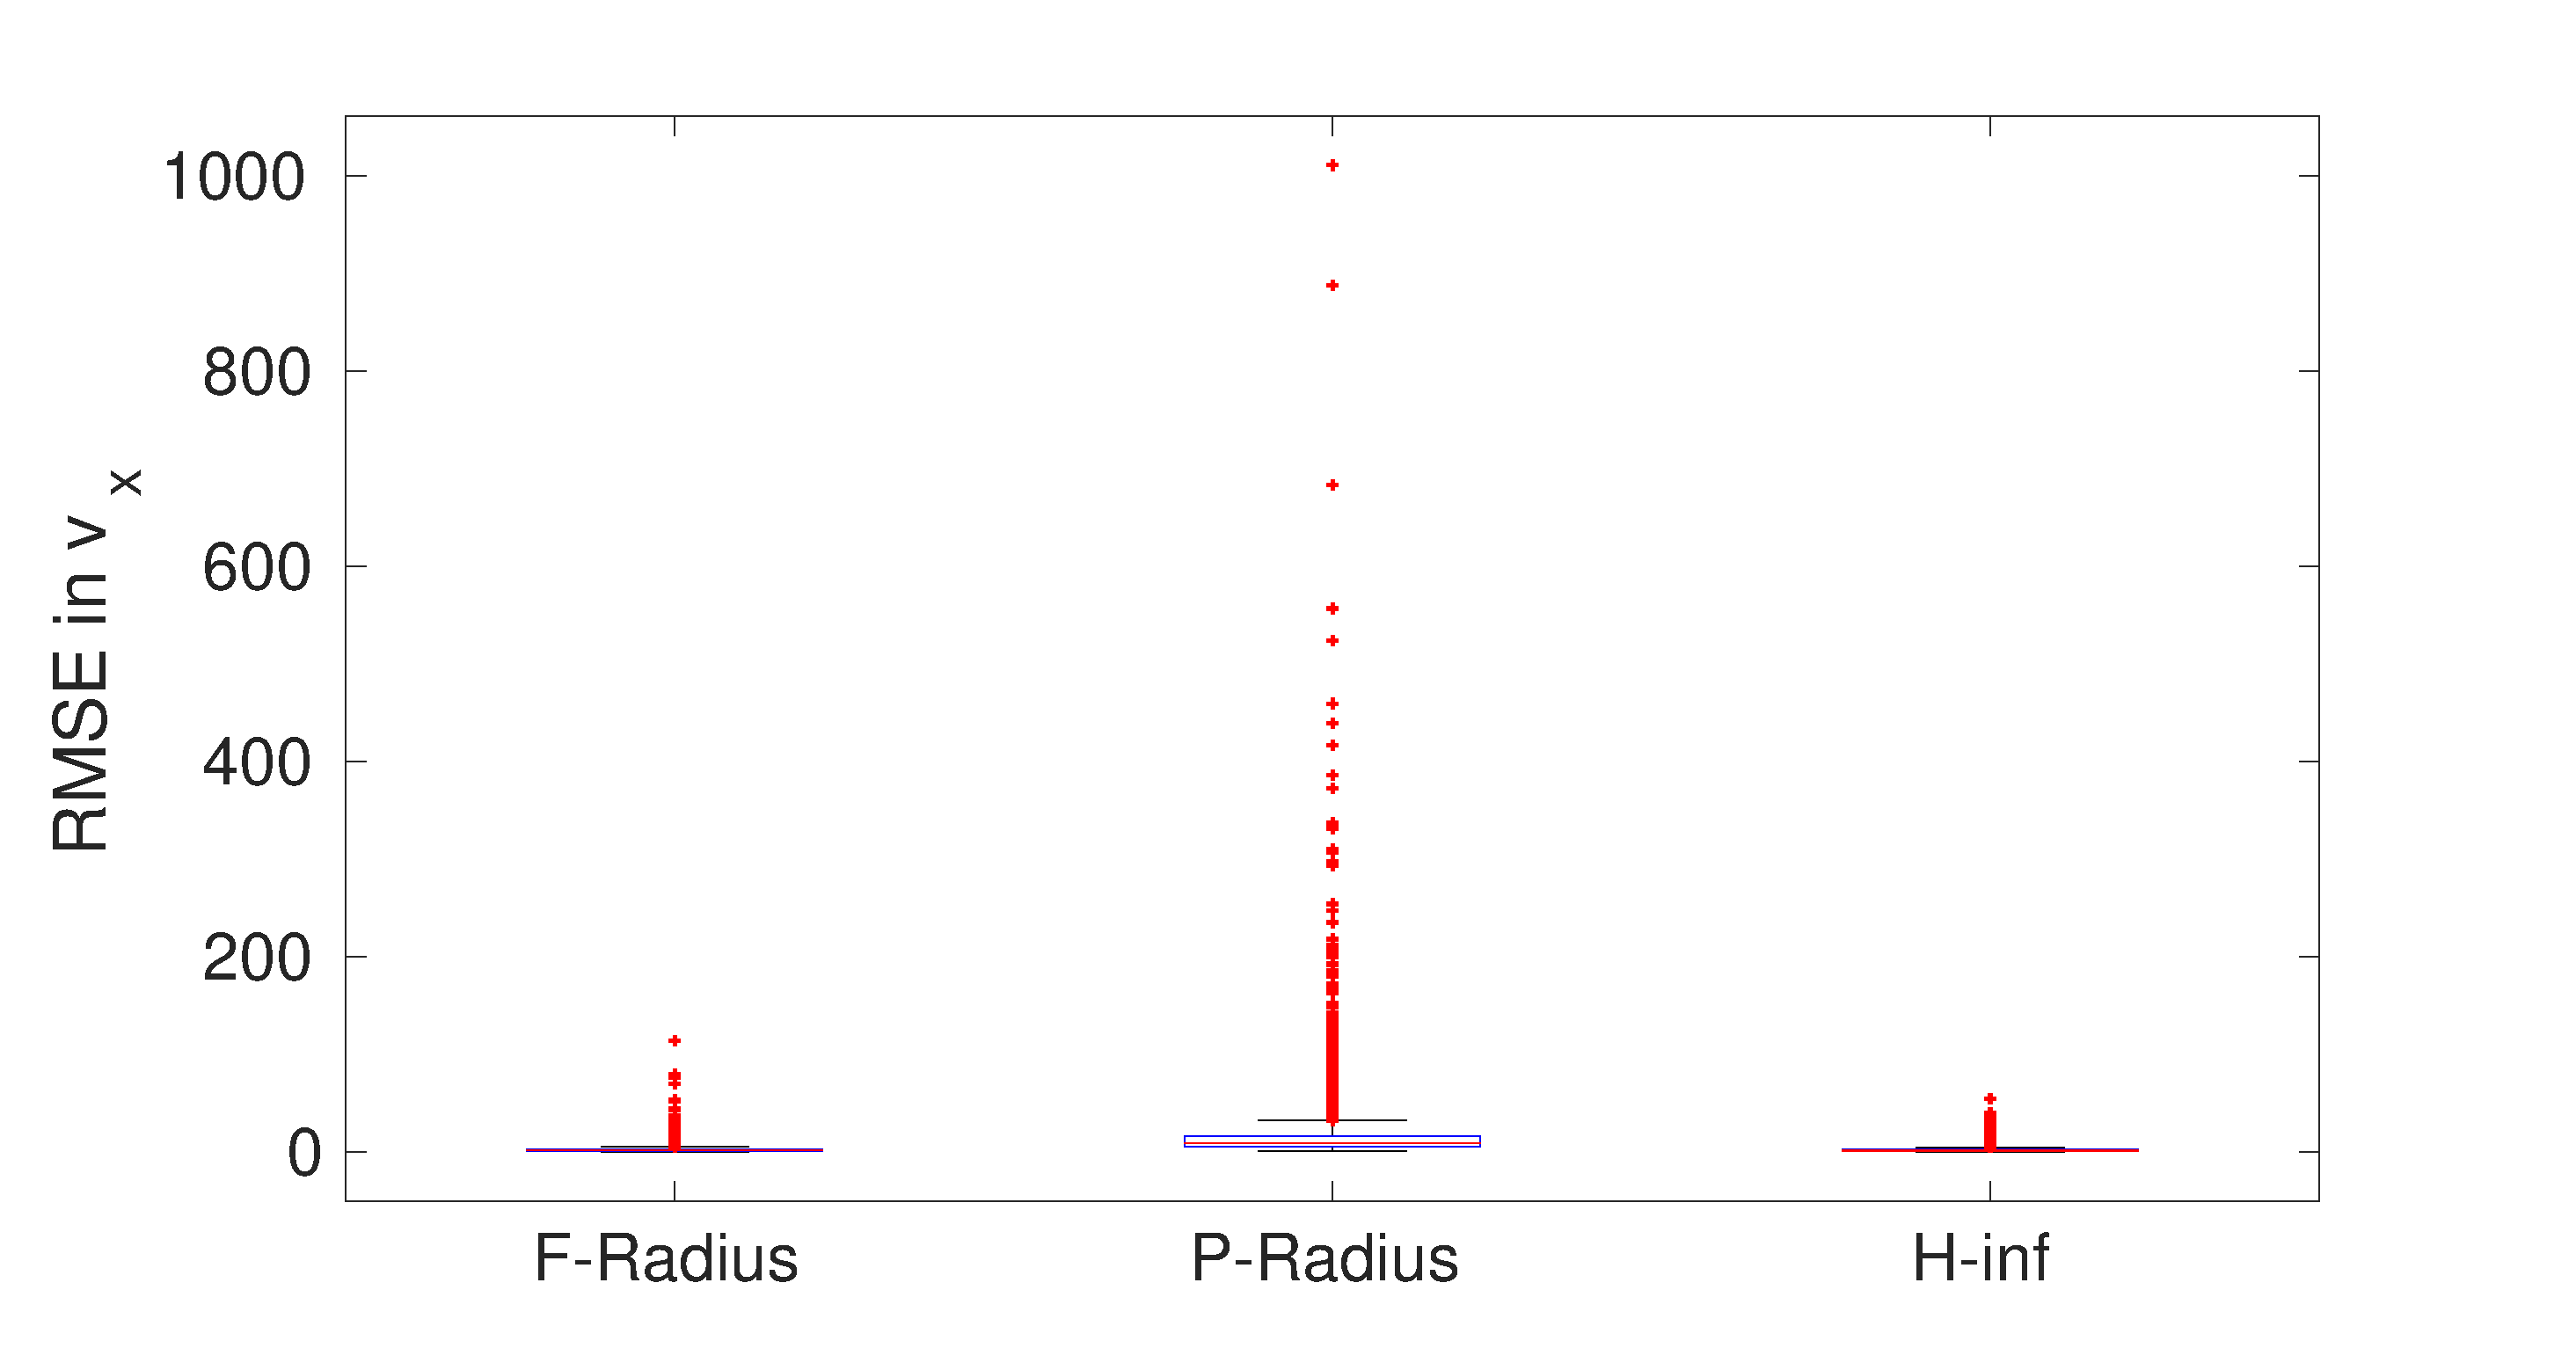
\includegraphics[width=\linewidth]{figures/Error/boxplotall}
\caption{RMSE(Root Mean Squared Error)}
\label{fig:boxplot}
\end{figure}

The boxplot of RMSE for $velocity_x$ using the point-mass model for all the techniques are shown in Fig. \ref{fig:boxplot}. The segment minimization using P-radius has a high range of extremes and the mean error is also greater than the other methods. The range of error is the lowest for H-$\infty$ observer with a mean 
1.9048 and a standard deviation of 1.9776 for $velocity_x$. A detailed report of the mean and standard deviation of each of the methods can be found in Tab. \ref{tab:errormean}. The error expectation from segment intersection optimizing F-radius is similar to H-$\infty$-based interval observer, however, the error in the measured state is slightly lesser in F-Radius compared to H-$\infty$ observer.


\begin{table}[!h]
\caption{Comparison of RMSE}
	\centering
	\renewcommand{\arraystretch}{1.1}
	\small	
	\begin{tabular}{l l l l l}
		\toprule 
		& \multicolumn{4}{c}{\textbf{Mean $\pm$ SD}} \\ \cmidrule{2-5}
		\textbf{Method} & \textbf{$s_x$} & \textbf{$s_y$} & \textbf{$v_x$} & \textbf{$v_y$}\\ \midrule
		%-------------------------------------		
		F-Radius & $0.0007\pm 0.0004$ &  $0.0004  \pm 0.0003$ &  $2.3412 \pm 2.7092$ &   $2.4184 \pm 1.5641$ \\
		P-Radius & $0.0016 \pm 0.0020$ &   $0.0008 \pm 0.0017$  & $13.4470 \pm 26.2465$ &  $13.7642 \pm 54.6724$\\
		H-$\infty$ approximation & $0.0007 \pm 0.0004$ &  $0.0006 \pm 0.0005$   & $1.9048 \pm  1.9776$  &  $ 2.1230 \pm  2.1946$\\
		%--------------------------------------		
		\bottomrule
	\end{tabular}
	\label{tab:errormean}
\end{table}

\section{Discussion}
The results in the previous sections show that every estimator has pros and cons. Besides, the output of the techniques depends heavily on the vehicle model used. In this section, we try to choose an estimator and a model, best suited to the collision avoidance system. 

Firstly, from the presented models, the point-mass model is the most accurate model for tracked vehicles, because it gives better estimates for acceleration. Secondly, comparing the estimators, the volume minimizer lost in computation time, whereas the P-radius minimizer gave terrible bounds. In contrast, the H-$\infty$-based observer computes the fastest, and the F-radius minimizer gave the tightest bounds with fewer measurements. The F-radius minimizer does not depend on the initial estimate. However, the computation time for F-radius rises with the dimension of the state. Moreover, adding constraints in F-radius also increases computation time. Although the computation time in Tab.~\ref{tab:comptime} for F-radius does not seem much in comparison to the time step (0.1s), the load would grow with the number of vehicles. In contrast, the H-$\infty$-based interval observer not only takes the shortest time, but also does not change with the increase in state dimension. Furthermore, it gives a lower range of error in estimation. However, one challenge with the H-$\infty$-based interval observer is to initialize the estimated state appropriately to ensure true state enclosure. This can be done in the collision avoidance system by adding the location of the ego vehicle and the maximum radius of the sensors. In conclusion, the H-$\infty$-based interval observer with pm model is the best choice for a collision avoidance system. 

%Time comparison for each method for n vehicles is shown in figure [cite]
%
%As seen from Fig. \ref{fig:segmentminimization}, the upper and lower bounds of the state estimation by Segment Intersection(using Frobenius norm) of the system bounds the true state. Comparing the error in different states of the system, as shown in Fig. \ref{fig:comparison}, suggests that all the algorithms require around 1s to converge to near the true state. Interesting to note, the Interval Estimation has a higher error peak compared to Segment Minimization using the same dataset.\\
%
%The Fig. \ref{fig:histogram} shows the Histogram of RMSE (Root Mean Square Error) of estimation from Segment Minimization. The errors are calculated after 10 seconds in order to avoid the initial peak. The histograms suggest that, the method gives little error for estimating the measured state, whereas, for unmeasured state like velocity, the error is at most twice the true state.


%\begin{figure}[h!]
%\begin{subfigure}{.5\textwidth}
%\centering
%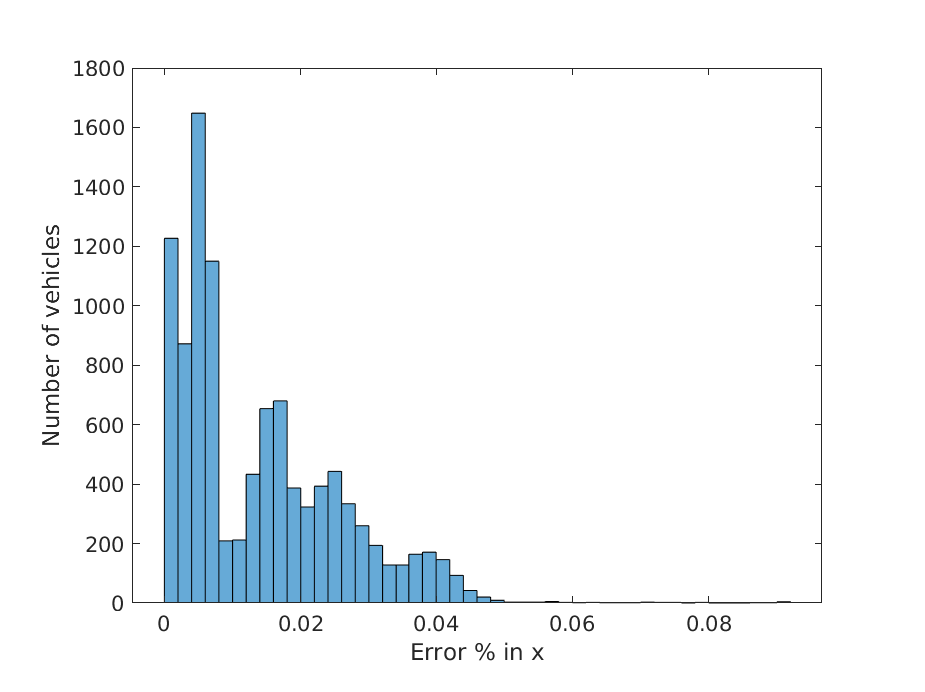
\includegraphics[width=.8\linewidth]{figures/s_caXerror}
%\caption{RMSE $x$}
%\end{subfigure}
%\begin{subfigure}{.5\textwidth}
%\centering
%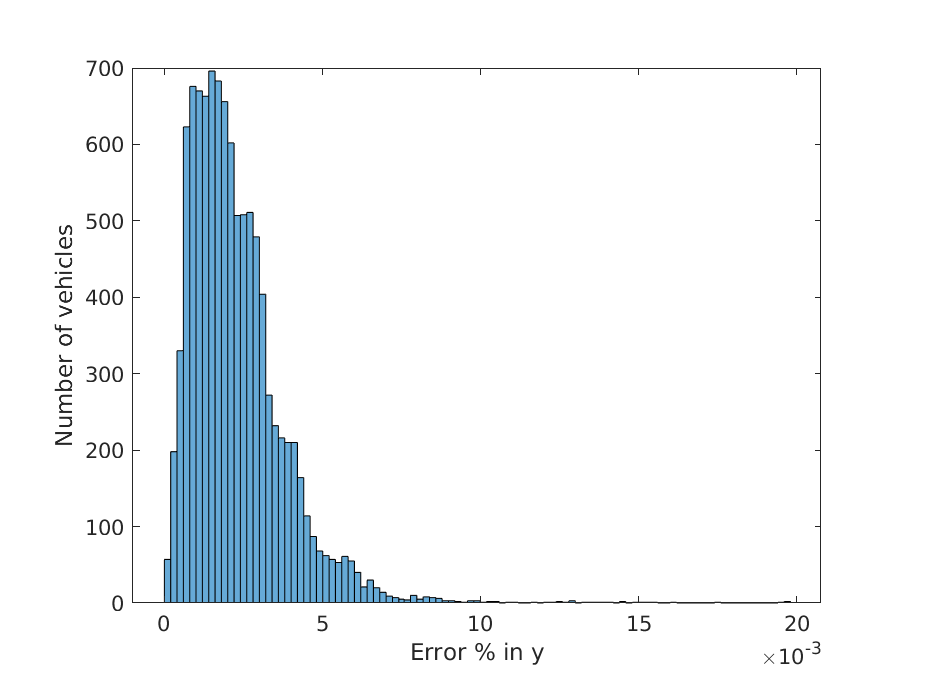
\includegraphics[width=.8\linewidth]{figures/s_caYerror}
%\caption{RMSE $y$}
%\end{subfigure}
%\begin{subfigure}{.5\textwidth}
%\centering
%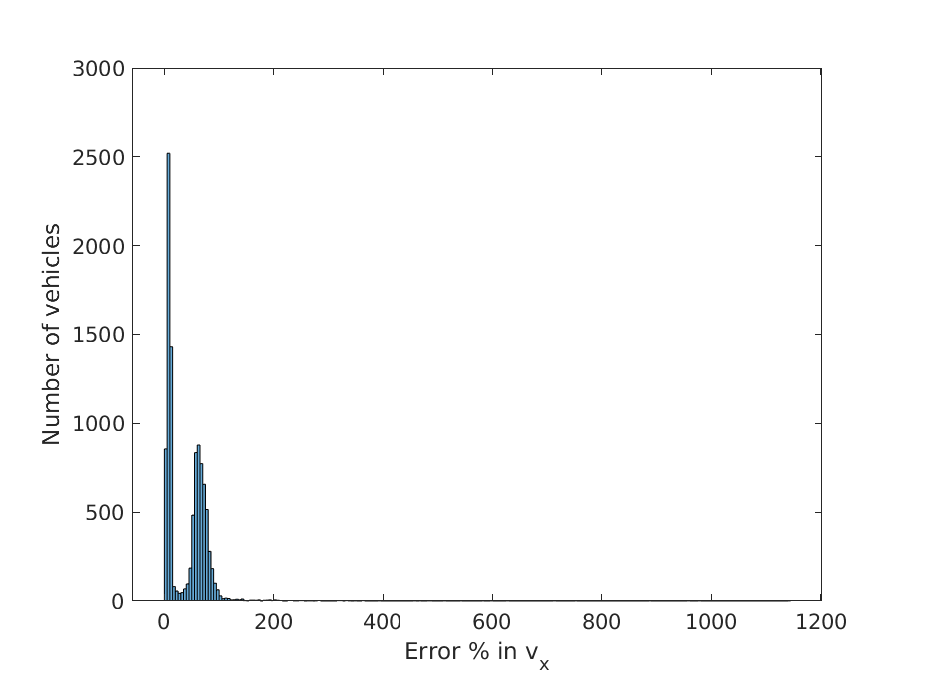
\includegraphics[width=.8\linewidth]{figures/s_cavXerror}
%\caption{RMSE in $velocity_x$}
%\end{subfigure}
%\begin{subfigure}{.5\textwidth}
%\centering
%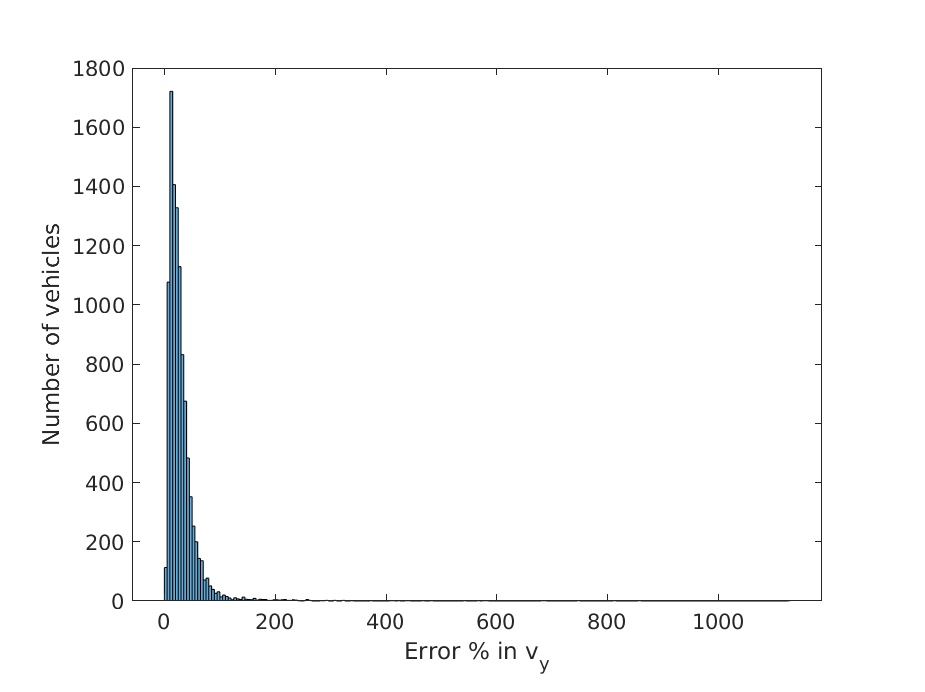
\includegraphics[width=.8\linewidth]{figures/s_cavYerror}
%\caption{RMSE in $velocity_y$}
%\end{subfigure}
%\caption{Histogram of errors from Segment Minimizer on 651 vehicles }
%\label{fig:histogram}
%\end{figure}
%\begin{itemize}
%\item{Efficiency}
%\item{Accuracy}
%\item{Performance Metric}
